\begin{figure}[htbp]
\centering
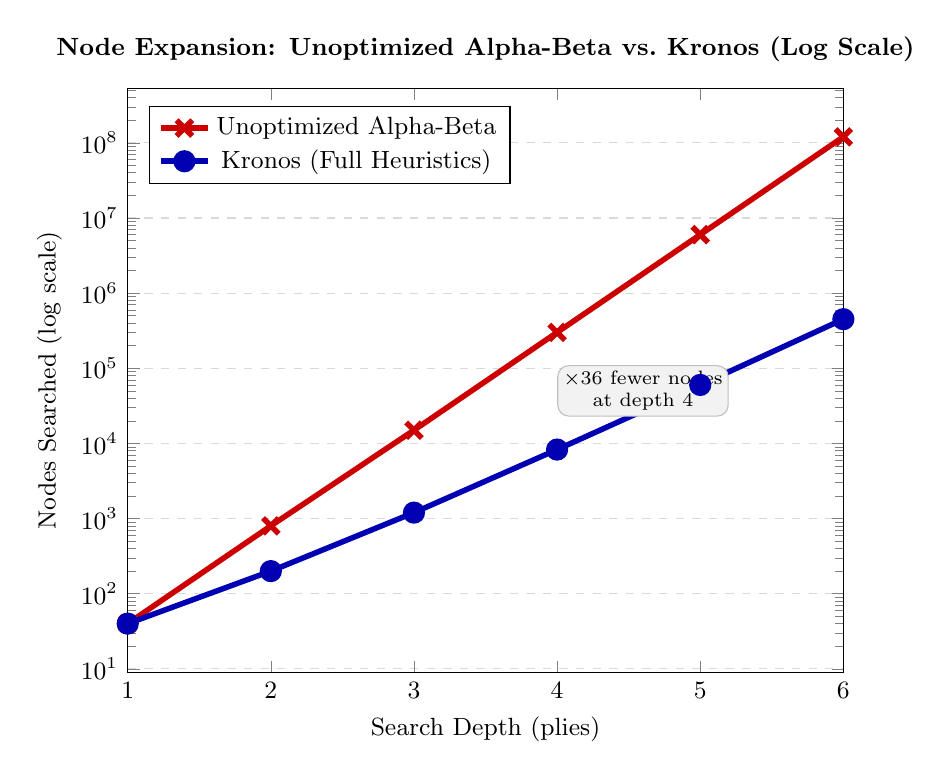
\begin{tikzpicture}
\begin{axis}[
    title style={font=\bfseries\small},
    title={Node Expansion: Unoptimized Alpha-Beta vs.\ Kronos (Log Scale)},
    xlabel={Search Depth (plies)},
    ylabel={Nodes Searched (log scale)},
    ymode=log,
    xmin=1, xmax=6,
    xtick={1,2,3,4,5,6},
    legend pos=north west,
    ymajorgrids=true,
    grid style={dashed, gray!30},
    width=0.88\textwidth,
    height=9cm,
    tick label style={font=\small},
    label style={font=\small},
    legend style={font=\small}
]
% Raw Alpha-Beta (no pruning or ordering)
\addplot[
    color=red!80!black,
    mark=x,
    mark size=4pt,
    line width=2pt
]
coordinates {
    (1, 40)
    (2, 800)
    (3, 15000)
    (4, 300000)
    (5, 6000000)
    (6, 120000000)
};
\addlegendentry{Unoptimized Alpha-Beta}

% Kronos full heuristics
\addplot[
    color=blue!70!black,
    mark=*,
    mark size=3pt,
    line width=2pt
]
coordinates {
    (1, 40)
    (2, 200)
    (3, 1200)
    (4, 8286)
    (5, 60000)
    (6, 450000)
};
\addlegendentry{Kronos (Full Heuristics)}

% Gap label at depth 4
\node[font=\scriptsize, fill=gray!10, draw=gray!50, rounded corners, inner sep=2pt, align=center]
    at (axis cs:4.6, 50000) {$\times$36 fewer nodes\\at depth 4};


\end{axis}
\end{tikzpicture}
\caption[Node Expansion Growth vs. Search Depth]{Exponential node expansion comparison between unoptimized Alpha-Beta and Kronos with all heuristics active (log scale). The unoptimized baseline represents search tree expansion without alpha-beta move ordering, whereas the optimized Kronos curve demonstrates the compounding impact of our full heuristic stack.}

\label{fig:node_growth}
\end{figure}
% Source Material: Benchmark ablation results at depth 4
